% Options for packages loaded elsewhere
\PassOptionsToPackage{unicode}{hyperref}
\PassOptionsToPackage{hyphens}{url}
\PassOptionsToPackage{dvipsnames,svgnames,x11names}{xcolor}
\documentclass[
]{article}
\usepackage{xcolor}
\usepackage[margin = 0.5in]{geometry}
\usepackage{amsmath,amssymb}
\setcounter{secnumdepth}{-\maxdimen} % remove section numbering
\usepackage{iftex}
\ifPDFTeX
  \usepackage[T1]{fontenc}
  \usepackage[utf8]{inputenc}
  \usepackage{textcomp} % provide euro and other symbols
\else % if luatex or xetex
  \usepackage{unicode-math} % this also loads fontspec
  \defaultfontfeatures{Scale=MatchLowercase}
  \defaultfontfeatures[\rmfamily]{Ligatures=TeX,Scale=1}
\fi
\usepackage{lmodern}
\ifPDFTeX\else
  % xetex/luatex font selection
\fi
% Use upquote if available, for straight quotes in verbatim environments
\IfFileExists{upquote.sty}{\usepackage{upquote}}{}
\IfFileExists{microtype.sty}{% use microtype if available
  \usepackage[]{microtype}
  \UseMicrotypeSet[protrusion]{basicmath} % disable protrusion for tt fonts
}{}
\makeatletter
\@ifundefined{KOMAClassName}{% if non-KOMA class
  \IfFileExists{parskip.sty}{%
    \usepackage{parskip}
  }{% else
    \setlength{\parindent}{0pt}
    \setlength{\parskip}{6pt plus 2pt minus 1pt}}
}{% if KOMA class
  \KOMAoptions{parskip=half}}
\makeatother
\usepackage{graphicx}
\makeatletter
\newsavebox\pandoc@box
\newcommand*\pandocbounded[1]{% scales image to fit in text height/width
  \sbox\pandoc@box{#1}%
  \Gscale@div\@tempa{\textheight}{\dimexpr\ht\pandoc@box+\dp\pandoc@box\relax}%
  \Gscale@div\@tempb{\linewidth}{\wd\pandoc@box}%
  \ifdim\@tempb\p@<\@tempa\p@\let\@tempa\@tempb\fi% select the smaller of both
  \ifdim\@tempa\p@<\p@\scalebox{\@tempa}{\usebox\pandoc@box}%
  \else\usebox{\pandoc@box}%
  \fi%
}
% Set default figure placement to htbp
\def\fps@figure{htbp}
\makeatother
\setlength{\emergencystretch}{3em} % prevent overfull lines
\providecommand{\tightlist}{%
  \setlength{\itemsep}{0pt}\setlength{\parskip}{0pt}}
\usepackage{color}
\usepackage{framed}
\setlength{\fboxsep}{.8em}

\usepackage{tcolorbox}

\tcbset{
  mystyle/.style={
    before skip=-10pt, % Adjust this value
    after skip=-10pt   % Adjust this value
  }
}
\newtcolorbox{mynoteblock}[1][]{mystyle, #1}

\newtcolorbox{blackbox}{
  colback=black,
  colframe=orange,
  coltext=white,
  boxsep=5pt,
  arc=4pt}
  
\newtcolorbox{ltbluebox}{
  colback=blue!5!white,
  colframe=blue!75!black,
  boxsep=5pt,
  arc=4pt}
  
\newtcolorbox{ltgreenbox}{
  colback=green!5!white,
  colframe=blue!75!black,
  boxsep=5pt,
  arc=4pt}
  
\newtcolorbox{ltpurplebox}{
  colback=purple!5!white,
  colframe=blue!75!black,
  boxsep=5pt,
  arc=4pt}
  


\newenvironment{cols}[1][]{}{}

\newenvironment{col}[1]{\begin{minipage}[t]{#1}\ignorespaces\vspace{0pt}}{%
\end{minipage}
\ifhmode\unskip\fi
\aftergroup\useignorespacesandallpars}

\def\useignorespacesandallpars#1\ignorespaces\fi{%
#1\fi\ignorespacesandallpars}

\makeatletter
\def\ignorespacesandallpars{%
  \@ifnextchar\par
    {\expandafter\ignorespacesandallpars\@gobble}%
    {}%
}
\makeatother

\usepackage{awesomebox}
\setlength{\aweboxvskip}{1mm}


\pagenumbering{gobble}

\usepackage{enumitem}
\setlist{itemsep=1pt, parsep=0pt} %# Adjust vertical spacing
\setlist[itemize,1]{leftmargin=*, labelsep=0.3em} %# Adjust horizontal spacing
\setlist[enumerate,1]{leftmargin=*, labelsep=0.3em} %# Adjust horizontal spacing

\usepackage{bookmark}
\IfFileExists{xurl.sty}{\usepackage{xurl}}{} % add URL line breaks if available
\urlstyle{same}
\hypersetup{
  colorlinks=true,
  linkcolor={Maroon},
  filecolor={Maroon},
  citecolor={Blue},
  urlcolor={blue},
  pdfcreator={LaTeX via pandoc}}

\author{}
\date{\vspace{-2.5em}}

\begin{document}

\vspace{-1cm}

\section{Spatial Measures: Potential Indicators and
Pathways}\label{spatial-measures-potential-indicators-and-pathways}

\begin{noteblock}
Spatial management encompasses both decision processes surrounding
delineation of management units (and how they correspond to stock units)
and also as a subset of measures setting, with area-based designations
for subsets of fishing activities. The spatial distributions of both
fishery resources and fishing fleets are dynamic and responsive to
multiple socio-economic and environmental drivers. Two cases were
identified for spatial measures implemented by the Council that could be
informed by ecosystem indicators: bycatch avoidance and establishing
habitat conservation areas.

\end{noteblock}

\begin{itemize}
\tightlist
\item
  \textbf{Key question: Can real time or projected habitat conditions
  assist with spatial measures setting??}
\item
  \textbf{Scope: demo for one species or develop a more general
  approach/process for all?}
\end{itemize}

\begin{cols}

\begin{col}{0.49\textwidth}

\begin{ltbluebox}

\subsection{What information is used
now?}\label{what-information-is-used-now}

The general process for setting spatial measures can be the same as for
all other measures as noted in the Measures Setting 1-pager. Measures
are set in specifications. The process for setting measures can be
changed by either FMP amendment or framework action.

\vspace{1ex}

The seasonal Scup Gear Restricted Areas (GRAs) are spatial measures
designed to reduce juvenile scup discards in small mesh fisheries. The
GRAs have remained the same for decades. They are currently being
\href{https://ccesuffolk.org/marine/fisheries/scup-gra}{re-evaluated}
using fishing and environmental data as well as industry expertise.

\vspace{1ex}

There are several current examples that use habitat indicators to
forecast bycatch potential in near-real time. The recently developed
\href{https://www.rhapcast.org/index.html}{RHAPcast} uses species
distribution model output and hindcast forecasts of habitat (sea surface
temperature) to identify areas that maximize target species encounters
while minimizing bycatch species encounters. This tool is similar to the
\href{https://oceanwatch.pifsc.noaa.gov/turtlewatch.html}{Turtlewatch}
approach in the Pacific.

\vspace{1ex}

\begin{center}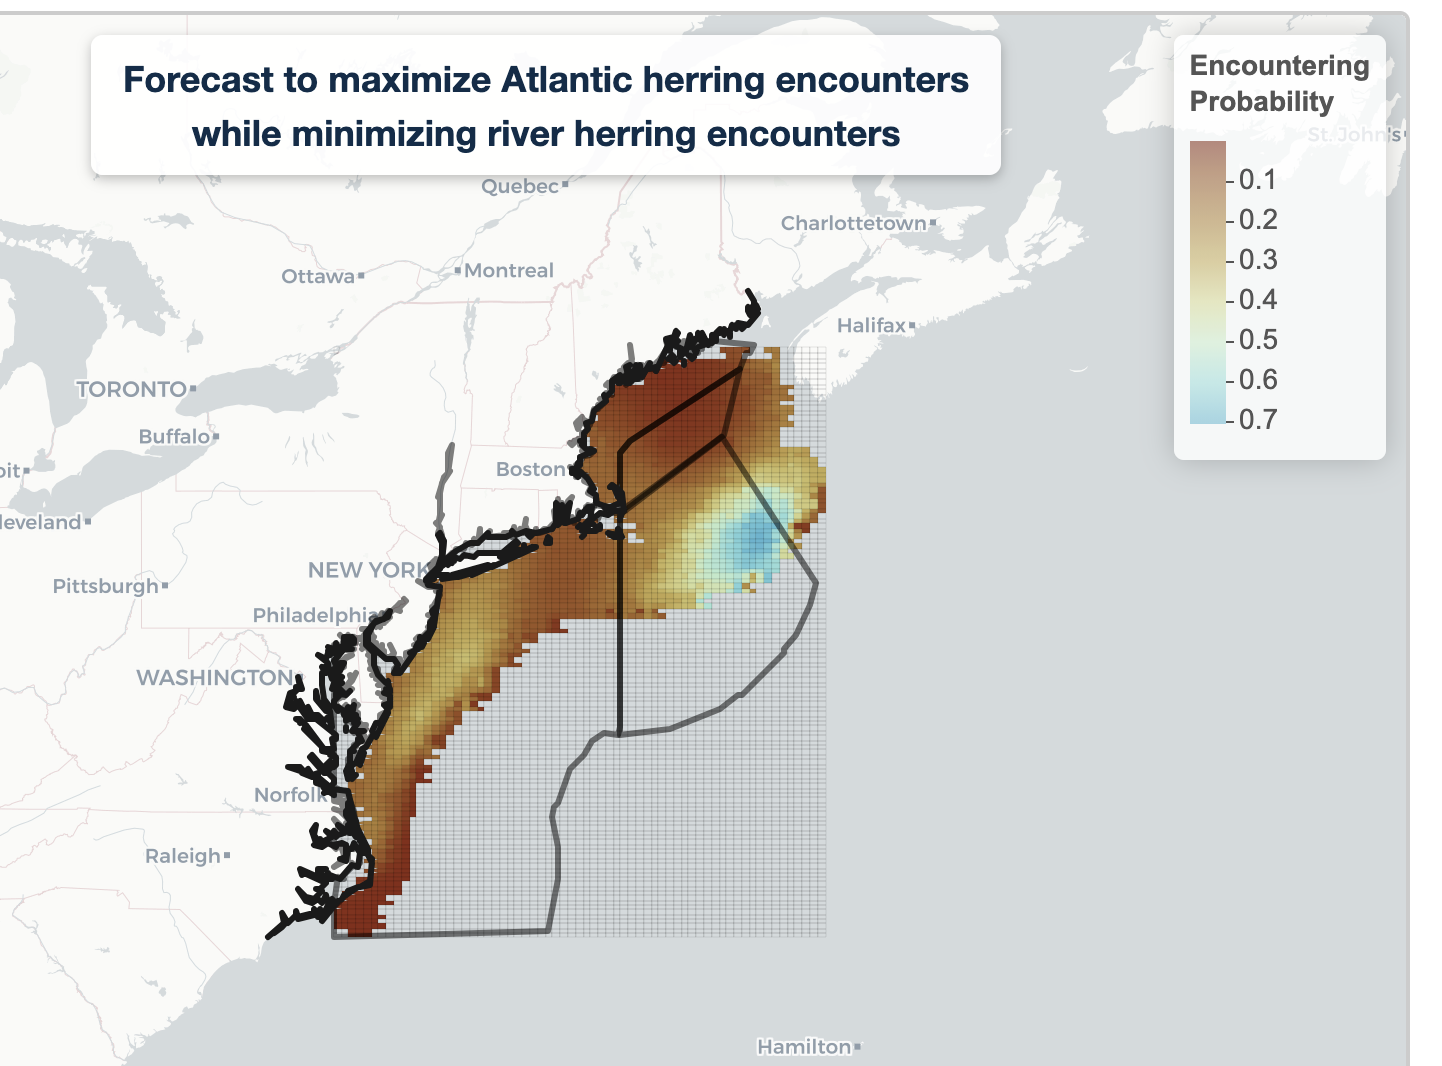
\includegraphics[width=0.87\linewidth]{rhapcast-screencap} \end{center}

\vspace{1ex}

Stock and fishery distribution shifts are also being addressed from a
\href{https://static1.squarespace.com/static/511cdc7fe4b00307a2628ac6/t/68e67a313a977f0b7ec34724/1759935025455/Project+7_IRA-Project-Brief.pdf}{governance
perspective}. Indicators developed for this project may also be useful
for developing and evaluating spatial measures.

\end{ltbluebox}

\end{col}

\begin{col}{0.02\textwidth}
~

\end{col}

\begin{col}{0.49\textwidth}

\begin{ltgreenbox}

\subsection{Information sources for
indicators}\label{information-sources-for-indicators}

\subsubsection{Potential Indicator
Sources}\label{potential-indicator-sources}

\begin{itemize}
\tightlist
\item
  Observer data bycatch estimates
\item
  Species distribution models and data products, e.g.~DisMAP (survey
  data) and NRHA data explorer
\item
  Spatiotemporal environmental forecasts from ocean model output
  (e.g.~MOM6)
\item
  Fishing effort distributions / footprints
\item
  Effects of Fishing database
\item
  \href{https://www.fisheries.noaa.gov/new-england-mid-atlantic/ecosystems/state-ecosystem-reports-northeast-us-shelf}{State
  of the Ecosystem} and
  \href{https://www.mafmc.org/s/2_MAB_RiskAssess_2024.pdf}{Risk
  Assessment} indicators
\end{itemize}

\subsubsection{Potential Pathways}\label{potential-pathways}

\textbf{Bycatch}

\begin{itemize}
\tightlist
\item
  Some spatial indicators could achieve management objectives for
  bycatch reduction if appropriate indicator information were made
  available to fishery participants so that they could decide how to
  avoid bycatch, rather than Council decisions.
\item
  Indicators of bycatch magnitude for certain areas could be monitored
  with respect to thresholds that would trigger spatial measures
\end{itemize}

\vspace{2ex}

\textbf{Establishing habitat conservation areas}

Once objectives for conservation areas are established, an analysis
could proceed by:

\begin{itemize}
\tightlist
\item
  Evaluate area measures with indicators of fishery and species spatial
  overlap:

  \begin{itemize}
  \tightlist
  \item
    Spatial distribution of fishery
  \item
    Spatial distribution of species
  \item
    Spatial model
  \end{itemize}
\item
  Determine habitat effects of fishing activity (e.g.~benthic impact
  studies)
\item
  Simulate relevant system drivers (species distribution shifts, fleet
  movement constraints, etc.)
\item
  Determine what spatial management measures meet objectives with
  minimal side effects?
\end{itemize}

\end{ltgreenbox}

\end{col}

\end{cols}

\begin{ltpurplebox}

\subsection{Information gaps}\label{information-gaps}

Spatial distribution of fishing effort may not be available/accessible
for all sectors / fleets. There are often challenges to map fishing
fleet effort to specific species, and with mismatches in spatial and
temporal scale of management areas and processes. Spatial measures also
have implications for future monitoring.

\end{ltpurplebox}

\end{document}
